% OpenAI Math Digest; layout adapted from the repository's Schnell diagrams.
\documentclass[border=12pt]{standalone}
\def\pgfsysdriver{pgfsys-dvisvgm.def}
\usepackage[dvisvgm]{xcolor}
\usepackage{xeCJK}
\setCJKmainfont{HaranoAjiGothic-Regular.otf}[BoldFont=HaranoAjiGothic-Bold.otf]
\setCJKsansfont{HaranoAjiGothic-Regular.otf}[BoldFont=HaranoAjiGothic-Bold.otf]
\usepackage{amsmath,amssymb,tikz,lmodern}
\usetikzlibrary{arrows.meta,positioning,calc}
\renewcommand{\familydefault}{\sfdefault}
\definecolor{ink}{HTML}{25322F}
\definecolor{green}{HTML}{246657}
\definecolor{tint}{HTML}{EEF4F0}
\definecolor{soft}{HTML}{C6D2CC}
\definecolor{muted}{HTML}{52615B}
\newif\ifJapanese
\newcommand{\Tx}[2]{\ifJapanese #1\else #2\fi}
\newcommand{\heading}[2]{{\color{green}\bfseries\Tx{#1}{#2}}\\[5pt]}
\newcommand{\refurl}[2]{\special{dvisvgm:raw <a xlink:href="#1" target="_blank" rel="noopener noreferrer">}{\setlength{\fboxsep}{0pt}\colorbox{white}{\color{green}\underline{\strut #2}}}\special{dvisvgm:raw </a>}}
\newcommand{\OI}[1]{\refurl{https://github.com/openai/math/blob/fd4aeeb2ee4fc729c18d98444fed42fd0529eeeb/preprints/Orbifold-and-logarithmic-Iitaka-subadditivity-September-26-2026/paper.pdf}{#1}}
\newcommand{\Fuj}[1]{\refurl{https://www.math.kyoto-u.ac.jp/~fujino/weak-posi11.pdf}{#1}}
\newcommand{\Cam}[1]{\refurl{https://arxiv.org/pdf/0705.0737v8}{#1}}
\tikzset{
 card/.style={draw=soft,fill=white,rounded corners=2pt,align=left,text=ink,font=\fontsize{10.5}{14}\selectfont,inner xsep=12pt,inner ysep=10pt,text width=14.4cm},
 half/.style={card,text width=6.35cm,minimum height=2.9cm},
 result/.style={card,draw=green,fill=tint,line width=.9pt},
 reason/.style={align=left,text=muted,font=\fontsize{9}{12}\selectfont,inner sep=0pt,text width=12.65cm},
 branchreason/.style={reason,text width=5.65cm},
 edge/.style={-{Stealth[length=2.4mm]},draw=green,line width=1pt},
 wire/.style={draw=green,line width=1pt},
}
% Every vertical arrow has a dedicated left gutter; all labels sit to its right.
\newcommand{\flow}[3]{
 \coordinate (#2-from) at ($(#1.south)+(-6.9,0)$);
 \coordinate (#2-to) at ($(#2.north)+(-6.9,0)$);
 \draw[edge] (#2-from)--(#2-to);
 \node[reason,anchor=west] at ($(#2-from)!.5!(#2-to)+(.55,0)$) {#3};
}

\Japanesetrue
\begin{document}
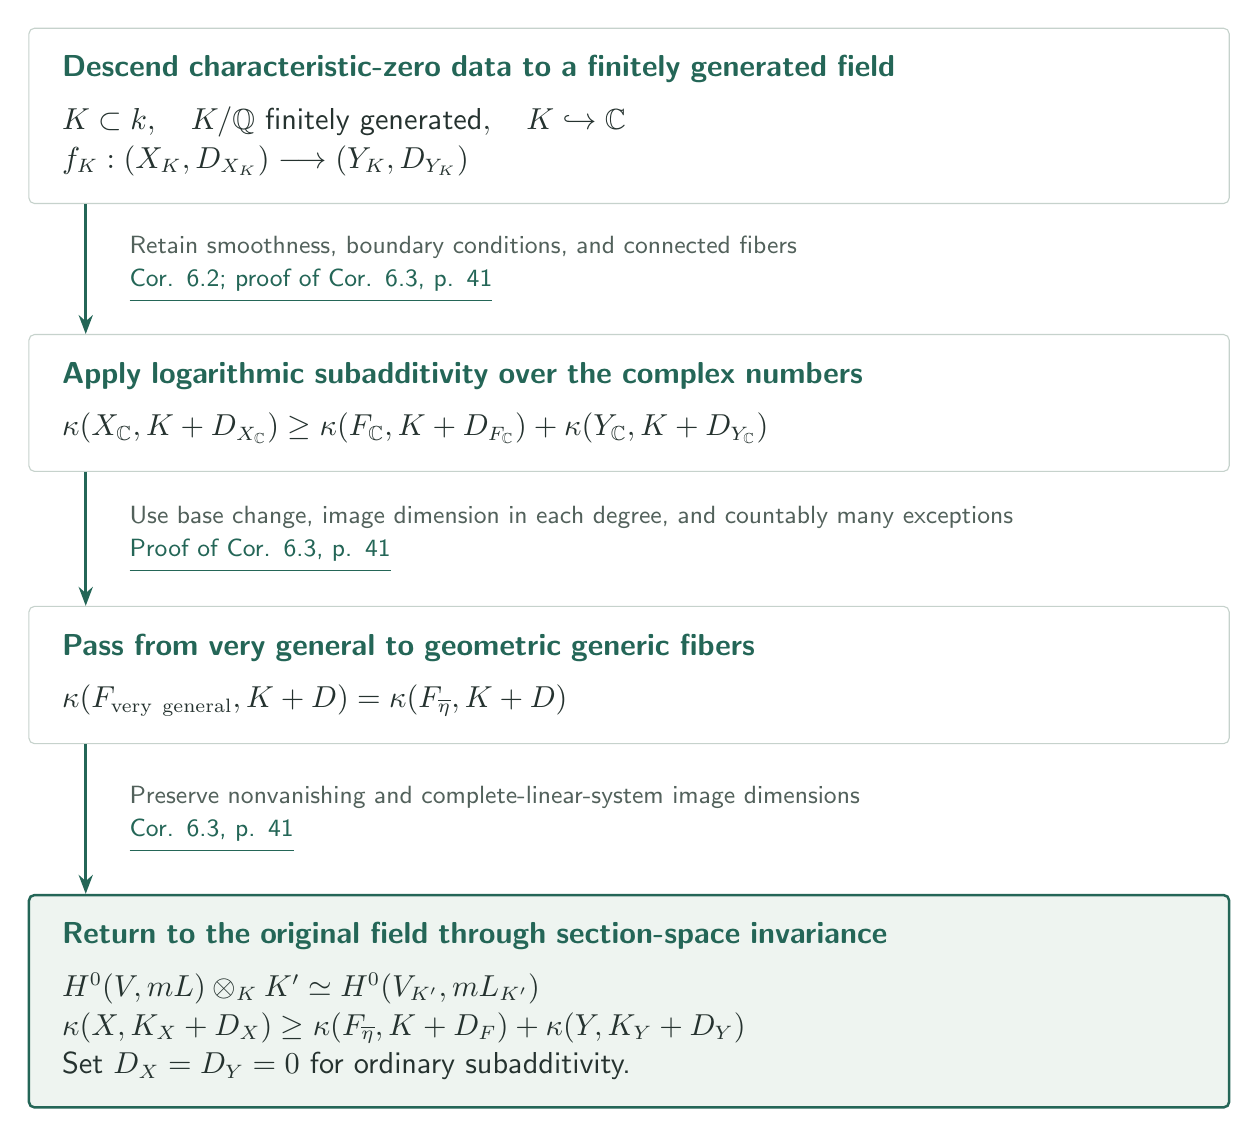
\begin{tikzpicture}
\node[card] (a) {\heading{標数0のデータを有限生成体へ降下}{Descend characteristic-zero data to a finitely generated field}
 $K\subset k,\quad K/\mathbb Q\ \text{finitely generated},\quad K\hookrightarrow\mathbb C$\\
 $f_K:(X_K,D_{X_K})\longrightarrow(Y_K,D_{Y_K})$};
\node[card,below=1.65cm of a] (b) {\heading{複素数上で対数不等式を適用}{Apply logarithmic subadditivity over the complex numbers}
 $\kappa(X_{\mathbb C},K+D_{X_{\mathbb C}})\ge
 \kappa(F_{\mathbb C},K+D_{F_{\mathbb C}})+\kappa(Y_{\mathbb C},K+D_{Y_{\mathbb C}})$};
\flow{a}{b}{\Tx{滑らかさ・境界条件・連結ファイバーを保持}{Retain smoothness, boundary conditions, and connected fibers}\\\OI{Cor. 6.2; proof of Cor. 6.3, p. 41}}
\node[card,below=1.7cm of b] (c) {\heading{非常に一般のファイバーから幾何学的一般ファイバーへ}{Pass from very general to geometric generic fibers}
 $\kappa(F_{\mathrm{very\ general}},K+D)
 =\kappa(F_{\overline\eta},K+D)$};
\flow{b}{c}{\Tx{各可除次数の基底変換と像の次元、可算個の例外集合を使う}{Use base change, image dimension in each degree, and countably many exceptions}\\\OI{Proof of Cor. 6.3, p. 41}}
\node[result,below=1.9cm of c] (d) {\heading{切断空間の体拡大不変性で元の体に戻す}{Return to the original field through section-space invariance}
 $H^0(V,mL)\otimes_KK'\simeq H^0(V_{K'},mL_{K'})$\\
 $\kappa(X,K_X+D_X)\ge\kappa(F_{\overline\eta},K+D_F)+\kappa(Y,K_Y+D_Y)$\\
 \Tx{$D_X=D_Y=0$で通常劣加法性}{Set $D_X=D_Y=0$ for ordinary subadditivity.}};
\flow{c}{d}{\Tx{非消滅と完備線形系の像の次元を保存}{Preserve nonvanishing and complete-linear-system image dimensions}\\\OI{Cor. 6.3, p. 41}}
\end{tikzpicture}

\end{document}
